\documentclass{article}
\usepackage{multirow,booktabs}
\usepackage{longtable}
\usepackage{eurosym}
%\usepackage{times}


\usepackage[margin=0.7in]{geometry}

\usepackage{array}
\newcolumntype{L}[1]{>{\raggedright\let\newline\\\arraybackslash\hspace{0pt}}m{#1}}
\newcolumntype{C}[1]{>{\centering\let\newline\\\arraybackslash\hspace{0pt}}m{#1}}
\newcolumntype{R}[1]{>{\raggedleft\let\newline\\\arraybackslash\hspace{0pt}}m{#1}}

\usepackage{siunitx} % Provides the \SI{}{} and \si{} command for typesetting SI units
\usepackage{graphicx} % Required for the inclusion of images
\usepackage{natbib} % Required to change bibliography style to APA
\usepackage{amsmath} % Required for some math elements 
\usepackage{appendix}

\setlength\parindent{0pt} % Removes all indentation from paragraphs

\renewcommand{\labelenumi}{\alph{enumi}.} % Make numbering in the enumerate environment by letter rather than number (e.g. section 6)


\title{Flow Sensors} % Title

\author{Nikesh \textsc{Bansal}} % Author name

\date{\today} % Date for the report


\begin{document}
	
	\begin{titlepage}
		
		%	LOGO SECTION
		%----------------------------------------------------------------------------------------
		
		\par
		\raisebox{-.5\height}{
\includegraphics[width=4cm]{projekt_9093.png}}%
		\hfill
		\raisebox{-.5\height}{
\includegraphics[width=4cm]{Logo_Uni_Freiburg.png}}\\[1 cm]%
		\par
		
		% Include a department/university logo - this will require the graphicx package
		
		%----------------------------------------------------------------------------------------
		
		\newcommand{\HRule}{\rule{\linewidth}{0.5mm}} % Defines a new command for the horizontal lines, change thickness here
		
		\center % Center everything on the page
		
		%----------------------------------------------------------------------------------------
		%	HEADING SECTIONS
		%----------------------------------------------------------------------------------------
		
		\textsc{\LARGE MST Design Lab I \\[0.5mm] WS 2016-17 }\\[1.5cm] % Name of your university/college
		\textsc{\Large Virtual Design Project}\\[0.5cm] % Major heading such as course name
		\textsc{\large "Energy-autonomous Embedded System "}\\[0.5cm] % Minor heading such as course title
		
		%----------------------------------------------------------------------------------------
		%	TITLE SECTION
		%----------------------------------------------------------------------------------------
		
		\HRule \\[0.4cm]
		%	\textsc{\large Experiment No. 3}\\[0.5cm]
		{ \huge \bfseries SMART BIKE PEDAL}\\[0.4cm] % Title of your document
		\HRule \\[1.5cm]
		
		%----------------------------------------------------------------------------------------
		%	AUTHOR SECTION
		%----------------------------------------------------------------------------------------
		\textsc{	Date : \today \\[1cm]
			\large	Group No. : 4 \\[1cm]
			\begin{flushleft}
				Authors: \\[0.5cm]
				1. Alireza (1111111) .............................. \\ [0.4cm]
				2. Jasleen (1111111) ..............................\\ [0.4cm]
				3. Mohseen (1111111) .............................. \\ [0.4cm]
				4. Nikesh (1111111) .............................. \\ [0.4cm]
				5. Taimoor (1111111) .............................. \\[0.4cm]
		\end{flushleft}}
		
		
		
		
		
		%   \begin{minipage}{0.4\textwidth}
		%		\begin{flushleft} \large
		%			\emph Group \textsc{2E}\\
		%			{Group Members: }\\
		%			Ahmad \textsc{Dbouk}\\
		%			Macit \textsc{Uluda}\\
		%			Nikesh \textsc{Bansal} % Your name
		%		\end{flushleft}
		%	\end{minipage}
		%	~
		%	\begin{minipage}{0.4\textwidth}
		%		\begin{flushright} \large
		%			\emph{Protocol Author:} \\
		%			Nikesh \textsc{Bansal}\\
		%			Matrikel-Nr. 4361939\\ 
		%			\vspace{5mm}
		%			{Date: }\\
		%			Decemeber 02,2016
		% Supervisor's Name
		%		\end{flushright}
		%	\end{minipage}\\[4cm]
		
		% If you don't want a supervisor, uncomment the two lines below and remove the section above
		%\Large \emph{Author:}\\
		%John \textsc{Smith}\\[3cm] % Your name
		
		%----------------------------------------------------------------------------------------
		%	DATE SECTION
		%----------------------------------------------------------------------------------------
		
		%{\large \today}\\[3cm] % Date, change the \today to a set date if you want to be precise
		
		%----------------------------------------------------------------------------------------
		
		\vfill % Fill the rest of the page with whitespace
		
	\end{titlepage}
	
	% If you wish to include an abstract, uncomment the lines below
	% \begin{abstract}
	% Abstract text
	% \end{abstract}
	
	\tableofcontents
	
	\newpage
	\listoffigures
	
	\vspace{2.5cm}
	\listoftables
	
	%----------------------------------------------------------------------------------------
	%	SECTION 1
	%----------------------------------------------------------------------------------------
	\newpage
	\section{Product Idea and Functions}
	
	\newpage
	\section{Market Situation}
	\subsection{Potential Market and Competitors}
	As per an article by bike-eu.com, the statistics show that in the year 2014, 133.1 million bicycles were sold resulting in the global cycling market of about € 35.7 billion. Thus, the average cost of a bicycle was approximately € 191 in 2014. The Europe alone contributed approximately € 12.8 billion which was 36\% of the global cycling market. A report ‘Growth Opportunities in the Global Bicycle Industry 2016-2021: Trends, Forecast, and Opportunity Analysis’ by Lucintel states that the global bicycle market is estimated to reach \$ 59.9 billion by the end of 2021. So, these statistics clearly show the increasing market for our product. \\
	Comment on increasing demand for bike accessories even more than new bikes (http://www.mintel.com/press-centre/leisure/mad-about-the-bike-sales-of-bicycle-accessories-outstrip-sales-of-bikes)\\[0.5cm]
	There is a French start-up ‘Connected Cycle’ which is working on the similar product and could be our competitor in the market. As per their website, the pedals will be launched in 2017. Their main dedication is to make the bikes and e-bikes fully connected to the smartphones, thus providing fitness tracking capabilities and location tracking facilities due to GSM and GPS modules inside their circuits. When the user starts pedaling, the sensors gets activated and the information regarding the location, speed and calories burned can be accessed by their connected cycle application. (which is yet to be launched)\\
	Connected Cycle successfully conducted an online crowdfunding campaign on Indiegogo.com. They were able to raise \$177,212 which was 188\% more than their target while selling their product for a early bird offer of \$189 for a pair of smart bike pedals.
	
	\subsection{Target Customers}
	Our product can be used by any bike-rider by replacing the normal pedals of the bike by our smart pedals. Also, our product can be used by those people who care about the environment but can’t switch to bicycles because they worry about their bicycles getting stolen. The main advantage would be the theft-protection, by being energy autonomous pedals, which normal bikes can’t offer. \\ 
	Many smart features in one product. \\ 
	Regular bike riders (more than once a week). Specially urban dwellers.
	
	\subsection{Evolution of Fitting Market}
	According to an article ‘Germany’s vicious cycle of bike thefts’ by ‘www.local.de’ on 17th July 2014, on an average 52\% German regularly ride the bike and there are 2.4 bicycles in every household. In the year 2013, a total of 317,000 bicycles were reported stolen in Germany and only 9.6\% of them were recovered. But many more bikes are stolen but not reported. Most of these stolen bikes are sold again in flea markets and on internet. As per the police, it’s easy to find the stolen car because of the unique number stamped on the engine but very few people take initiative to get a unique number framed for their bikes, which will make it easy to find the stolen bike.\\  
	Increasing number of smart bike accessories and their demand and also increasing number of bikes leads to more demand.
	
	
	
	
	
	
	\newpage
	\section{Fabrication Cost and Sales numbers}
	
	\subsection{Comparable Products}
	In the below table, a number of well-known products are mentioned which share their function with the product proposed in this document. The current price of these products are also cited approximately with their corresponding deviation. We must however note that despite the last product, connected cycle®, all other products mentioned in the below table have completely separate functions from each other. Yet, the last one is a pedal which covers some of the functions of the other products. Namely, this pedal is used for bike-theft protection and also for presenting statistical information such as speed and distance for fitness purposes. [?mentioning where we have got these prices values from][??picture for connected cycle?]\\
	
	\begin{table}[h]
		\begin{center}
			\begin{tabular}{|C{6cm}|C{3cm}|C{4cm}|}
				\hline
				Available Products & Average Cost & Cost Deviation  \\
				\hline
				Conventional Bike Pedals & \euro 15 & \euro 5\\
				\hline
				Bicycle back-light sets & \euro 10 & \euro 5\\
				\hline
				Bicycle speedometers & \euro 15 & \euro 10\\
				\hline
				Popular bicycle locks & \euro 40 & \euro 20 \\ 
				\hline
				Bicycle dynamo & \euro 30 & \euro 5 \\
				\hline
				Connected cycle & \euro 170 & \euro 30 \\
				\hline
				
				
			\end{tabular}
			\caption{Product Costs}
		\end{center}
	\end{table}
	
	
	\subsection{Selling Price Estimation}
	The products remarked in the above table cover a number of functions, all of which are included in the product which is proposed in this document. There is already a considerable number of customers who buy a complete set of the above products (excluding Connected cycle, and pedals) for their bicycles and spent nearly 95 euros. Therefore, if the price of our product is below this number and if we can indeed make our customers confident enough that our product is satisfactory as a substitute of the above products, we can be confident about the absolute willingness of the customers for buying it. However, we have also observed a quite a large market demand for this new product of Connected cycle pedals which charges its customers nearly 170 euros for a pair of pedals. Therefore, with respect to the extra functions which our product presents in comparison to all the above examples, and by taking into account the available market demand, we can be confident about selling this product if the price is below 170 euros, and also to outcompete the similar producers in the market. In addition, the current bicycle manufacturers can also additionally, be our potential customers who can consider this product as a substitute for the conventional embedded pedals to attract more customers in selling their bicycles. Here, the price of this pedal can be more flexible upwards with respect to price of the bicycle itself. Furthermore, the local governments who are willing to either monitor the bike traffic or manage bicycle fleets can offer subsidy for this product. On the other hand, the fact that how much a customer would be willing to pay for this product also depends on the price of his own bicycle. Generally, for bicycle users who already have the aforementioned products, it can be the additional feature of our product, namely, being smart, that can be compelling for buying it.  
	
	
	\subsection{Sales Number Estimation}
	As an example, in Europe which is one of the best potential markets, about 20 million new bicycles were sold on 2014. Here, an ideal case would be if all the customers of these bicycles consider our product an appealing substitute for not buying locks, light sets, dynamos, and speedometers, besides achieving additional functions. Therefore, maximum the same number can be the number of sales in such year. However, as the customers’ view can be rather subjective, we can only say that it greatly depends on the price of our product and how much we can attract our customers to this product for how much the sales number will be. We must also note the degree of availability of our product in the market, and how many of the new bicycle owners notice our product as other factors in our sales number. \\ 
	Similarly, as aforementioned, approximately 130 million bicycles (adult bicycle?) were sold on 2014 in the world []. Here, the price of our product plays a greater role for how much our sales number can be as our customers’ ability to afford it deviates in a broader range than Europe. Above all, with respect to the feedbacks which we get from the market in the initial phases of presenting our product we can make a better approximation about this matter. \\
	In addition, the connected cycle has already sold ….. number. Therefore, with respect to how better our product is visualized in the market, our sales number can also be expected between this number and a half of it.
	
	\begin{figure}[h!]
		\begin{center}
			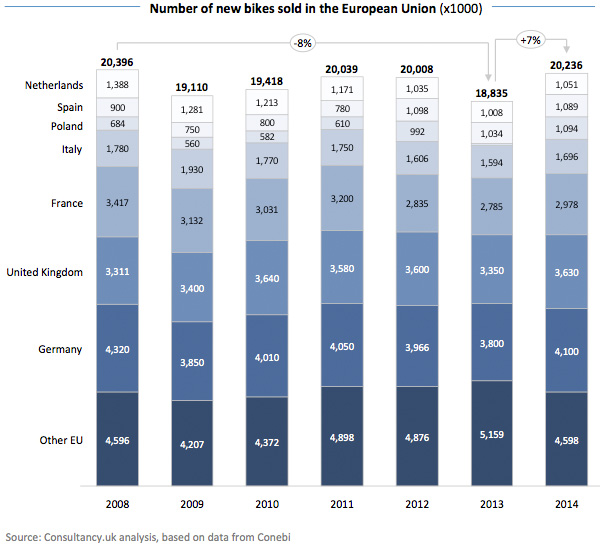
\includegraphics[width=0.45\textwidth]{3_3_new_bikes.jpg} % Include the image placeholder.png
			\caption{Number of new bikes sold in European Union}
		\end{center}
	\end{figure}
	
	
	\subsection{Target Places}
	Initially, we would like to aim some of the most bike-friendly cities and countries where the number of bicycle riders are relatively high and the price of our product can be considered reasonable for customers. Namely, Germany, Switzerland, Netherlands, Denmark, France, England, Ireland, USA, Canada, China, Russia and etc. are examples of such countries. After receiving our feedbacks from the market and customers, and perhaps, modifying our product we can consider a broader range of countries to present this product in. In addition, as the manufacturing rate of our product increases we might be able to decrease the price and sell in countries where our new prices can be considered more affordable. [refrence?]
	
	
	\subsection{Fabrication Cost}
	The main parts included for fabrication of this product are as follows: \\[1cm]
	
	\begin{table}[h]
		\begin{center}
			\begin{tabular}{|C{9cm}|C{2cm}|}
				\hline
				\bfseries{Product} & \bfseries{Cost}\\ 
				\hline
				IMU (Accelerometer and Gyroscope) & \euro 15\\
				\hline
				GSM Module & \euro 20\\ 
				\hline
				GPS Module & \euro 15\\
				\hline
				Sound buzzer & \euro 5 \\ 
				\hline
				Light emiiting diodes (LEDs) (50 pieces) & \euro 5 \\ 
				\hline
				Rechargeable battery & \euro 5\\ 
				\hline
				Electromotor & \euro 10\\ 
				\hline
				Sum & \euro 75\\
				\hline
				
			\end{tabular}
			\caption{Cost of parts}
		\end{center}
	\end{table}
	
	
	\newpage
	
	\begin{table}
		\centering
		\caption[SPECIFICATION SHEET]{}
		\vspace{0.5cm}
		\begin{tabular}{|L{4cm}|C{9cm}|L{4cm}|}
			\hline 
			\multicolumn{3}{ |c| }{ SPECIFICATION SHEET} \\
			\hline 
			\multirow{3}{3.5cm}{Uni Freiburg/IMTEK Lab course „MST Design Lab I“} & \multirow{5}{7cm}{Project Name: Smart Bike Pedal}  &   \\
			& & Version: \\
			& & Pages Total: \\
			Semester: & & Delivery Date: \\
			Group No.: & & \\
			\hline    
		\end{tabular}
		\begin{tabular}{|L{8.719cm}|L{8.719cm}|}
			Contact person / The customer givin you the & Contact person / You as a company \hfill   \\ 
			development task & receiving the development task \\
			& \\
			& \\
			& \\
			& \\
			\hline
		\end{tabular}
	\end{table}
	\begin{longtable}{|C{1cm}|C{2cm}|L{9.56cm}|L{4cm}|}
		RWO & Change Date & Description & Response \\
		\hline
		
		& & \textbf{Part III. General Attributes} & \\
		\hline
		& & 1. Geometry & \\
		R & & \hspace{1mm} 1.1 Length : 70 $\pm$ 5 mm & \\
		R & & \hspace{1mm} 1.2 Width : 80 $\pm$ 5 mm & \\
		R & & \hspace{1mm} 1.3 Height : 25 $\pm$ 3 mm & \\
		R & & \hspace{1mm} 1.4 Mass of a pair of bike pedals = 450 $\pm$ 50 grams & \\
		W & & \hspace{1mm} 1.5 Mass of a pair of bike pedals = 300 $\pm$ 50 grams & \\
		\hline
		& & 2. Kinematics & \\
		R & & \hspace{1mm} 2.1 Rotation in plane parallel to plane of bike with threshold force of 20 $\pm$ 2 N at the edge of the pedal & \\ 
		\hline
		& & 3. Force & \\
		R & & \hspace{1mm} 3.1 Max. force applied by the person on bike pedal = 2500 $\pm$ 50 N & \\
		\hline
		& & 5. Matter & \\
		R & & \hspace{1mm} 5.1 Top and bottom surfaces should have tread surface & \\
		R & & \hspace{1mm} 5.2 Should pass xxxxxxxxx test & \\
		R & & \hspace{1mm} 5.3 waterproof, dust proof, humidity proof, temperature resistive & \\
		\hline
		& & 7. Safety & \\
		R & & \hspace{1mm} 7.1 Environment Standard - look up? & \\
		R & & \hspace{1mm} 7.2 Charge protection & \\
		R & & \hspace{1mm} 7.3 Voltage protection  & \\
		R & & \hspace{1mm} 7.4 Battery compartment locked by safety mechanism (suggestion : computerized mechanical key) & \\
		R & & \hspace{1mm} 7.5 Soft reset for electronic system and hard reset in battery compartment & \\
		
		\hline
		& & 8. Ergonomy & \\
		R & & \hspace{1mm} 8.1 Curved edges & \\
		R & & \hspace{1mm} 8.2 Change of battery using push-in mechanism & \\
		
		\hline		
		
		& & 9. Production & \\
		R & & \hspace{1mm} 9.1 Fabrication technology & \\
		& & \hspace{1mm} 9.2 & \\
		\hline
		& & 10. Control & \\
		& & \hspace{1mm} 10.1 Should pass ISO 4210-8:2014 test & \\
		& & \hspace{1mm} 10.2 & \\
		& & \hspace{1mm} 10.3 & \\
		\hline
		& & 11. Mounting & \\
		R & & \hspace{1mm} 11.1 Pedal Threads = 9/16 inches $\times$ 20 tpi & \\
		R & & \hspace{1mm} 11.2 Metal  & \\
		R & & \hspace{1mm} 11.3 Test standard & \\
		R & & \hspace{1mm} 11.4 Head profile - Hexagonal & \\
		\hline
		
		& & 12. Transport & \\
		
		R & & \hspace{1mm} 12.1 Transport -- ISO 17365:2013  & \\
		R & & \hspace{1mm} 12.2 Distribution packaging -- ISO 780:2015 & \\
		\hline
		
		\multicolumn{4}{|l|}{} \\
		\multicolumn{4}{|l|}{Legend to RWO:} \\
		\multicolumn{4}{|l|}{R = Requirement} \\
		\multicolumn{4}{|l|}{W = Wish (Priority can be set 1-2-3)} \\
		\multicolumn{4}{|l|}{O = Option} \\
		
		\hline
		
		
		& & 13. Packaging & \\
		R & & \hspace{1mm} 13.1 Packaging -- ISO 17366:2013 & \\
		R & & \hspace{1mm} 13.2 Dimension of box = l x b x h & \\
		R & & \hspace{1mm} 13.3 2 lock keys for battery compartment & \\
		R & & \hspace{1mm} 13.4 1 battery  & \\
		R & & \hspace{1mm} 13.5 2 bike pedals wrapped separately with wrapping material  & \\
		R & & \hspace{1mm} 13.6 1 User manual  & \\
		\hline
		& & 14. Use & \\
		R & & \hspace{1mm} 14.1 Electronics noise safe level $<$ 30 dB & \\
		R & & \hspace{1mm} 14.2 Wear = ??? & \\
		R & & \hspace{1mm} 14.3 As bike pedals & \\
		R & & \hspace{1mm} 14.4 Temperature : -20 $\pm$ 1$^{\circ}$C to 60 $\pm$ 1$^{\circ}$C  & \\
		R & & \hspace{1mm} 14.5 Use standards -- IP6, IP7, CE & \\
		\hline
		& & 15. Software Application & \\
		R& & 15.1 Software application to show data for speed, acceleration. etc.& \\
		\hline 
		& & 16. Maintainance & \\
		R & & \hspace{1mm} 16.1 Maintainance -- free & \\
		R & & \hspace{1mm} 16.2 Exchange battery : 2-3 years & \\
		\hline
		& & 17. Recycling & \\
		R & & \hspace{1mm} 17.1 Re-usable as a normal bike pedal & \\
		R & & \hspace{1mm} 17.2 Standards for recycling electronics and battery & \\
		\hline
		& & 18. Cost & \\
		R & & \hspace{1mm} 18.1 Maximum cost : \euro 100 & \\
		\hline
		& & 19. Dates & \\
		R & & \hspace{1mm} 19.1 Duration of development : Summer semester & \\		 
		\hline
		& & \textbf{Part I. Left hand side Pedal Attributes} & \\
		\hline
		& & 4. Energy & \\
		R & & \hspace{1mm} 4.1 Energy autonomous & \\
		R & & \hspace{1mm} 4.2 Battery standby time = 3-4 weeks & \\
		R & & \hspace{1mm} 4.3 Active life time of battery = 48 hours & \\
		R & & \hspace{1mm} 4.4 Battery life cycle = 2-3 years & \\
		R & & \hspace{1mm} 4.5 Voltage of system = 3.3 - 3.6 V & \\
		\hline
		& & 6. Signal & \\
		R & & \hspace{1mm} 6.1 Front and back surface should have red LED panels  &  \\
		W & & \hspace{1mm} 6.1 Front  surface should have white LED panel and back surface should have red LED panel  &  \\
		R & & \hspace{1mm} 6.2 Signal for location of bike & \\
		R & & \hspace{1mm} 6.3 Signal for communication with mobile phone & \\
		R & & \hspace{1mm} 6.4 Speed, Acceleration and turn detection & \\
		R & & \hspace{1mm} 6.5 Send log data & \\
		R & & \hspace{1mm} 6.6 Sound alarm for theft protection & \\
		\hline
		& & 7. Safety & \\
		R & & \hspace{1mm} 7.1 Environment Standard - look up? & \\
		R & & \hspace{1mm} 7.2 Charge protection & \\
		R & & \hspace{1mm} 7.3 Voltage protection  & \\
		R & & \hspace{1mm} 7.4 Battery compartment locked by safety mechanism (suggestion : computerized mechanical key) & \\
		R & & \hspace{1mm} 7.5 Soft reset for electronic system and hard reset in battery compartment & \\
		\hline
		& & 11. Mounting & \\
		R & & \hspace{1mm} 11.5 Thread profile = Left-hand side & \\
		\hline
		& & \textbf{Part II. Right hand side Pedal Attributes} & \\
		\hline
		& & 4. Energy & \\
		W & & \hspace{1mm} 4.1 Rechargable battery (Suggestion : The battery is charged by wires in lock) &  \\
		W & & \hspace{1mm} 4.2  &  \\
		\hline
		& & 6. Signal & \\
		W & & \hspace{1mm} 6.1 Front and back surface should have red LED panels  &  \\
		W & & \hspace{1mm} 6.1 Front  surface should have white LED panel and back surface should have red LED panel  &  \\
		\hline
		
		\hline
		& & 11. Mounting & \\
		R & & \hspace{1mm} 11.1 Thread profile = Right-hand side   & \\
		\hline	  
		
	\end{longtable} 
	
	
	
	
	
	
	
	
	
\end{document}